\documentclass[conference]{IEEEtran}
\IEEEoverridecommandlockouts
\usepackage{cite}
\usepackage{amsmath}
\usepackage{graphicx}
\usepackage{booktabs}
\usepackage{url}

\newcommand{\pmtwofive}{PM\textsubscript{2.5}}

\begin{document}

\title{Deep Neural Networks for \pmtwofive{} Air-Quality Estimation from Street-Level Images: Project Proposal and Literature Overview}

\author{
\IEEEauthorblockN{Ahamed Hasan}
\IEEEauthorblockA{\textit{OsloMet}\\
ahhas2658@oslomet.no}
\and
\IEEEauthorblockN{Mrinmoy Das}
\IEEEauthorblockA{\textit{OsloMet}\\
mrdas1414@oslomet.no}
\and
\IEEEauthorblockN{Mughilvannan Manivannan}
\IEEEauthorblockA{\textit{OsloMet}\\
muman2187@oslomet.no}
}

\maketitle

\begin{abstract}
This report contains two parts, project proposal and literature review. We propose a deep neural network (DNN) that can estimate the \pmtwofive{} air quality index (AQI) from a single street-level image. The DNN is trained using 11,114 labelled images. The literature review analyses and summarises Kamble \textit{et al.} (IEEE Access 2025), a lightweight deep-learning framework that estimates \pmtwofive{} from smartphone photos and Razimi \textit{et al.} (IEEE SCOReD 2024), a hybrid model combining VGG16 deep learning with classical colour and texture analysis to classify digital images.
\end{abstract}

\begin{IEEEkeywords}
deep learning, convolutional neural networks, air quality, \pmtwofive{}, image regression, haze
\end{IEEEkeywords}

\section{Task 1: Group Project Proposal}

\subsection{Tentative Title}
\textit{Sky-Aware Deep Neural Networks for Estimating \pmtwofive{} Air Quality from Street-Level Photographs.}

\subsection{Project Idea}
Fine particulate matter scatters sunlight. Hazy air therefore lowers contrast, washes out colour and brightens the darkest parts of a scene. These are cues that are visible in an ordinary image. We will train a deep neural network that predicts \pmtwofive{} AQI from a street-level photo using these cues. The network has two branches: a pre-trained convolutional neural network (CNN) fine-tuned on the image, and a small multilayer perceptron (MLP) on interpretable haze features measured separately on the sky and ground regions. The model is then tested on images that are not seen during training, and Grad-CAM~\cite{selvaraju2017} is used to check that the network tends to the haze cues rather than the scene's content. Three questions guide our work: (RQ1)~which haze cues and image regions the network relies on; (RQ2)~whether fusing hand-crafted haze features with CNN features improves accuracy at unseen images; and (RQ3)~how much location and season metadata impacts the training, and whether the image remains useful once they are included.

\subsection{Why It Matters}
Fine particulate matter is among the most harmful air pollutants, yet reference monitoring stations are expensive and sparse, so most places have no local reading. Cameras and smartphones, by contrast, are everywhere. A reliable image-based estimator would give low-cost, high-density estimates, and fill gaps between stations. Also, it can help people understand the air-quality in their neighbourhood easily. In practice, such a model could power a phone app that turns a snapshot into a local health warning. Explainability matters as much as accuracy, because users and authorities must be able to trust that the estimate reflects haze rather than scenery. Scientifically, the project tests whether deep networks learn physically meaningful haze cues and whether they generalise to new locations, a known weakness of current models~\cite{byler2025}.

\subsection{Brief Literature Review}
Classical dehazing explains why photos carry this information: the dark channel prior~\cite{he2011} shows that haze lifts the darkest pixel values of a scene. Recent work (Table~\ref{tab:lit}) builds on such cues but leaves clear gaps. Kamble \textit{et al.}~\cite{kamble2025} feed frozen EfficientNet features of smartphone photos to a BiLSTM and add weather data, but use one camera view in one city. Han \textit{et al.}~\cite{han2025} train a contrastive network on fixed traffic cameras that needs as few as 50 labelled images per camera, but assumes a static background. Lee and Moses Manova~\cite{lee2025} show that near-infrared and red-edge drone bands separate haze from cloud, raising three-level accuracy from 95.1\% to 99.6\% on private data. Byler \textit{et al.}~\cite{byler2025} find that image models exceed 80\% accuracy at seen sites but reach at most 65\% at unseen ones. SkyFuseNet~\cite{abdelsalam2026} fuses a Swin transformer with station readings and reports $R^2=0.998$, but its image branch alone fails (RMSE 158.95), so its accuracy comes from the sensor inputs. The gaps are (i)~small single-site datasets, (ii)~little evaluation at unseen locations, and (iii)~fusion with pollutant readings that would not exist at deployment.

\begin{table*}[t]
\centering
\caption{Recent IEEE Work on Image-Based \pmtwofive{} Estimation}
\label{tab:lit}
\begin{tabular}{p{3.9cm}p{3.4cm}p{4.3cm}p{4.3cm}}
\toprule
Work & Images & Network & Main limitation \\
\midrule
Kamble \textit{et al.}~\cite{kamble2025}, IEEE Access 2025 & Smartphone, one fixed view & EfficientNet-B1 + BiLSTM + weather & Single site, consumer-sensor labels \\
Han \textit{et al.}~\cite{han2025}, IEEE Access 2025 & Fixed traffic cameras & Contrastive ResNet18 & Static scenes only \\
Lee and Moses Manova~\cite{lee2025}, IEEE Sens.\ J.\ 2025 & Drone RGB + multispectral & Dual-channel CNN with attention & Private data, split not reported \\
Byler \textit{et al.}~\cite{byler2025}, WACVW 2025 & Park webcams, 15 sites & ResNet101 + location embedding & Large drop at unseen sites \\
Abdelsalam and Sayed~\cite{abdelsalam2026}, IMSA 2026 & Smartphone sky photos & Swin-S + sensor MLP & Relies on PM\textsubscript{10} sensor input \\
\bottomrule
\end{tabular}
\end{table*}

\subsection{Dataset}
We use PM25Vision~\cite{pm25vision}: 11,114 Mapillary street-level photos (2014--2025) labelled with the \pmtwofive{} AQI (1--530) of 3,261 World Air Quality Index stations, released under CC~BY~4.0. After removing duplicates and 18 images that appear in both splits, 8,176 training and 2,920 test images remain, and training and test stations are disjoint. The photos come from handheld cameras and dashcams with very different viewpoints. Labels are strongly regional and seasonal (median AQI from 28 in Oceania to 142 in Asia, with winter peaks), and only 4\% of images exceed AQI 300, so high-pollution cases are rare. The NPS-AQI webcam dataset~\cite{byler2025} is a candidate for out-of-domain testing.

\subsection{Approach and Model}
\begin{itemize}
\item \textit{Haze branch:} six filters (dark channel~\cite{he2011}, saturation, brightness, blue ratio, Sobel edges, local contrast) are pooled over the top, middle and bottom thirds of the image with the mean and 10th/90th percentiles (54 features), followed by an MLP.
\item \textit{Image branch:} EfficientNet-B0~\cite{tan2019} pretrained on ImageNet, fine-tuned on the full image and on a sky crop.
\item \textit{Head:} the branch embeddings are concatenated and fed to a regression head (Huber loss on $\log(1+\mathrm{AQI})$) with an auxiliary AQI-category head and sample weights for rare high-AQI images, to counter regression to the mean.
\item \textit{Training:} Adam with early stopping; only flips and small crops are used for augmentation, because colour jitter would alter the haze cue itself.
\item \textit{Evaluation:} five-fold cross-validation grouped by station, final testing on unseen stations, and MAE, RMSE, $R^2$ and Spearman $\rho$ against a median baseline, with branch and metadata ablations.
\item \textit{Success criteria:} the fused network should beat both the median baseline and the linear baselines in Section~\ref{sec:prelim} on unseen stations, and Grad-CAM should place most attention on the sky and distant scene rather than on cars or buildings.
\end{itemize}

\subsection{Preliminary Work: EDA and Feature Extraction}
\label{sec:prelim}
We have already explored the data and extracted features~\cite{nbeda,nbfeatures}, for two reasons: to make the evaluation trustworthy, and to find which visual cues the network should exploit. The exploratory data analysis (EDA) removed duplicate and leaking labels and showed that 7,596 images share a station and day with another image, so all validation must be grouped by station. For feature extraction, each filter was pooled over the three image bands and ranked by its rank correlation with AQI and by the cross-validated error of a linear network. Haze filters carry most of their signal in the sky band ($|\rho|\approx0.26$, Fig.~\ref{fig:heatmap}). On unseen test stations, a linear network on the 54 filter features reached $R^2=0.18$ (MAE 54.9 versus 63.6 for the median baseline), and a linear head on frozen EfficientNet-B0 embeddings reached $R^2=0.30$. Month and location alone reached $R^2=0.60$, so metadata will be reported separately to keep the contribution of the image visible. These results justify the two-branch design and set the baselines that the final network must beat.

\begin{figure}[t]
\centering
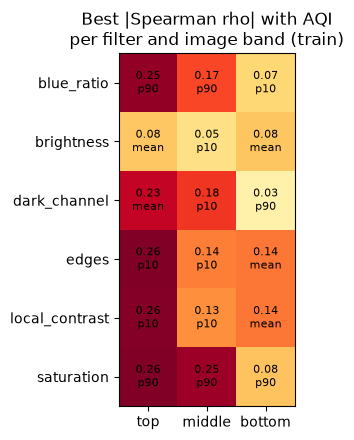
\includegraphics[width=0.75\columnwidth]{figures/filter_band_heatmap.png}
\caption{Best Spearman $|\rho|$ between each haze filter and AQI per image band (training set), with the statistic that achieves it.}
\label{fig:heatmap}
\end{figure}

\section{Task 2: Literature Overview}

\subsection{1st Paper}
A.~Kamble, S.~Aramkul and P.~Champrasert, ``A Mobile Image-Driven \pmtwofive{} Estimation Framework Using Deep Learning Techniques,'' \textit{IEEE Access}, vol.~13, 2025~\cite{kamble2025}.

\subsection{Extended Summary}
Northern Thailand suffers severe \pmtwofive{} episodes during the burning season, and Chiang Mai lies in a valley where polluted air dissipates slowly. Government stations are few, so the authors ask whether a phone photo can estimate the concentration at a specific place cheaply and quickly.

They built their own dataset (CMU). One fixed view in Chiang Mai was photographed with a smartphone in the morning, afternoon and evening from December 2021 to June 2022. Each shot was taken in both HDR and non-HDR mode, giving 442 images per set; HDR was included because it preserves detail in both the bright sky and the dark foreground, where haze is most visible. Labels came from a portable Xiaomi \pmtwofive{} sensor at the same spot (2--98.4~$\mu$g/m$^3$), and temperature, wind speed and humidity from the nearest station through the IQAir AirVisual app. A second set (DTU, Delhi) has 369 images taken five minutes apart over four days.

The framework has two stages. A CNN pretrained on ImageNet turns each image into a feature vector, with all layers frozen except the last. A two-layer bidirectional LSTM (BiLSTM, hidden size 32) then regresses the \pmtwofive{} value. EfficientNet-B0 to B3 and ResNet-18/50 backbones are compared with LSTM and BiLSTM heads. The Met- variant appends the three weather values to the 1,280-dimensional EfficientNet feature vector. Models are trained with Adam (learning rate $5\times10^{-4}$, batch size 16) for 500 epochs (1,000 with weather) on a shuffled 80/20 split, and scored with MAE, SMAPE and Pearson's $r$. Besides accuracy, the authors measure computational cost as parameters and floating-point operations per image, which matters for deployment on phones.

EfficientNet-B1 (7.79M parameters, 0.69 GFLOPs) beat ResNet-18 (11.69M, 1.81 GFLOPs) in both accuracy and cost, while the larger B2 and B3 were worse. Shuffling improved every model, HDR images gave slightly lower errors than non-HDR images, and weather inputs gave further gains (Table~\ref{tab:kamble}).

\begin{table}[t]
\centering
\caption{Key Results of Kamble \textit{et al.}~\cite{kamble2025}, EfficientNet-B1-BiLSTM (MAE in $\mu$g/m$^3$)}
\label{tab:kamble}
\footnotesize
\begin{tabular}{lccc}
\toprule
Dataset and split & MAE & SMAPE (\%) & $r$ \\
\midrule
CMU, time order kept & 14.60 & 55.9 & 0.50 \\
CMU, shuffled & 8.2 & 31 & 0.61 \\
CMU, shuffled + weather & 7.6 & 29 & 0.68 \\
DTU, shuffled & 5.3 & 10.8 & 0.91 \\
DTU, shuffled + weather & 4.06 & 8.3 & 0.94 \\
\bottomrule
\end{tabular}
\end{table}

\subsection{Analysis of Three Main Points}
\textit{1) Lightweight transfer learning suits small data.} Freezing a pretrained EfficientNet and training only a small recurrent head keeps the number of trainable parameters low, which limits overfitting on 442 images and makes on-device inference realistic. That B2 and B3 performed worse than B1 shows that a larger backbone does not help when data are scarce. Reporting parameters and FLOPs next to accuracy is a strength, since it makes the accuracy--cost trade-off explicit. The limitation is that ImageNet features are tuned to objects, whereas haze is a global, low-level change in contrast and colour that a frozen backbone cannot adapt to. With about 8,000 images, our project can fine-tune deeper layers, and our frozen-embedding baseline ($R^2=0.30$) shows how much signal generic features already carry.

\textit{2) Weather fusion helps only modestly.} Adding temperature, wind speed and humidity lowered MAE on CMU from 8.2 to 7.6~$\mu$g/m$^3$, an improvement the authors themselves call marginal; temperature alone gave about half of the gain. These single-variable ablations are good practice, and we will repeat them for our metadata. Three values are simply concatenated with 1,280 image features, so the network can easily ignore or overweight them. Weather data must also be available at prediction time, which a phone app can only provide through an online service. Our preliminary MLP showed the opposite imbalance: metadata alone predicted AQI far better than the image features, and plain concatenation reduced accuracy. We will therefore use separate branches and always report image-only results, so the contribution of the image stays visible.

\textit{3) The evaluation limits the generalisation claim.} All images show one scene, labels come from a consumer sensor, and the 80/20 split is random over a time series. Neighbouring frames, taken minutes apart with almost the same \pmtwofive{} level, can fall on both sides of the split. This probably explains why shuffling improved results so strongly (CMU MAE from 14.60 to 8.2; DTU $r$ from $-0.22$ to 0.91). Shuffling also removes the temporal order that a BiLSTM is designed to exploit, which the authors acknowledge when noting that temporal dependency was hard to learn from small datasets. No test on another camera or location is reported, although image models are known to degrade at unseen sites~\cite{byler2025}. A blocked split, for example holding out whole days or weeks, would give a more honest estimate of performance under new conditions. Our station-disjoint splits and grouped cross-validation are designed to avoid this optimism.

Overall, the paper shows that an efficient CNN with a small recurrent head can estimate \pmtwofive{} from phone photos and that auxiliary weather data can help. Its evidence, however, comes from a single scene. For our work, the paper motivates the EfficientNet backbone and the auxiliary-input design, while its weaknesses motivate our station-disjoint evaluation across thousands of locations.

\subsection{2nd Paper}
U.~N.~A. Razimi, A.~M. Ali, and R.~Osman, ``Integrating Deep Learning Features Extraction and Image Processing for Visual Pattern Analysis in Air Quality Index (AQI) Classification,'' in \textit{Proc. IEEE 22nd Student Conf. Res. Develop. (SCOReD)}, 2024~\cite{razimi2024}.

\subsection{Extended Summary}
While deep convolutional networks can extract complex abstract features from images, traditional image processing techniques are highly effective at capturing specific low-level visual indicators like color degradation and texture blurring caused by pollution. Razimi \textit{et al.} explore whether combining these two approaches can improve the classification of images into six discrete AQI categories (ranging from ``Good'' to ``Severe''). 

The authors utilized a Kaggle dataset comprising 12,240 daytime images collected from 16 distinct locations across India and Nepal. Their methodology employs a two-pronged feature extraction strategy. First, they use a pre-trained VGG16 network (excluding the top classification layers) to extract high-level spatial and structural features from resized $224 \times 224$ images. Second, they explicitly extract classical image features by converting the images to grayscale to compute Local Binary Pattern (LBP) histograms for texture, and by calculating the average red, green, and blue (RGB) pixel values for color characteristics. 

These deep and classical features are concatenated and fed into a Fully Connected Neural Network (FCNN) possessing three dense layers, appropriately regularized by batch normalization and dropout. They trained two FCNN variants: Model 1 (using only VGG16 features) and Model 2 (the hybrid approach). The hybrid model achieved an overall accuracy of 93\%, reflecting a 3\% improvement over the VGG16-only baseline. Model 2 showed particularly strong performance gains in identifying the extreme ``Good'' and ``Severe'' categories, demonstrating that explicitly providing color and texture cues helps the network distinguish varying levels of atmospheric haze.

\subsection{Analysis of Three Main Points}
\textit{1) Hybrid feature extraction overcomes backbone limitations.} Pre-trained ImageNet models like VGG16 are optimized to detect distinct objects (e.g., animals, vehicles), whereas air pollution is an environmental condition that manifests globally as reduced light intensity and contrast. By explicitly appending average RGB values and LBP texture histograms, the authors inject crucial domain-specific cues that the deep network might otherwise struggle to learn or prioritize. This directly validates our project's proposed two-branch architecture, which similarly fuses pre-trained CNN embeddings with hand-crafted haze filters (dark channel, blue ratio) to ensure the model focuses on atmospheric scattering rather than just scene content.

\textit{2) Latent space visualization confirms feature separability.} The authors use t-SNE dimensionality reduction to visualize the extracted hybrid features in a 2D space. The resulting plot shows distinct clustering for the different AQI classes, visually confirming that the model has learned meaningful representations. However, they also noted overlapping clusters, particularly between adjacent categories like ``Moderate'' and ``Unhealthy for Sensitive Groups.'' We can adopt a similar t-SNE or PCA visualization step in our own methodology to verify whether our chosen haze features successfully group high-AQI and low-AQI images before classification.

\textit{3) Framing AQI as a classification task creates artificial boundaries.} The paper treats AQI estimation as a strict 6-class classification problem. The authors observe that misclassification primarily occur between adjacent classes due to visual similarities. This overlap is natural because AQI is fundamentally a continuous variable; an AQI of 50 (Good) looks nearly identical to an AQI of 51 (Moderate), yet a classifier forces this boundary into a hard split. This observation strongly supports our project's decision to treat AQI estimation as a continuous regression problem using Huber loss. Regression naturally accommodates the continuous degradation of visibility caused by particulate matter without forcing artificial categorical thresholds.

Overall, the paper shows that fusing deep CNN embeddings with classical handcrafted image features improves AQI classification compared to relying on deep learning alone. Its evidence, however, is limited to categorizing images into broad pollution classes on a dataset where spatial overlap and class confusion still exist.

\begin{thebibliography}{00}
\bibitem{pm25vision} ``PM25Vision: A large-scale benchmark dataset for visual estimation of air quality,'' arXiv:2509.16519, 2025.
\bibitem{kamble2025} A. Kamble, S. Aramkul, and P. Champrasert, ``A mobile image-driven PM2.5 estimation framework using deep learning techniques,'' \textit{IEEE Access}, vol. 13, 2025, doi: 10.1109/ACCESS.2024.3521966.
\bibitem{razimi2024} U. N. A. Razimi, A. M. Ali, and R. Osman, ``Integrating deep learning features extraction and image processing for visual pattern analysis in air quality index (AQI) classification,'' in \textit{Proc. IEEE 22nd Student Conf. Res. Develop. (SCOReD)}, 2024, doi: 10.1109/SCOReD64708.2024.10872648.
\bibitem{han2025} Y. Han, V. O. K. Li, J. C. K. Lam, S. Song, and T. Mo, ``SmartCamAirDetect: A contrastive approach for probabilistic ambient air pollution estimation with limited images for smart city development,'' \textit{IEEE Access}, vol. 13, pp. 121073--121085, 2025, doi: 10.1109/ACCESS.2025.3583794.
\bibitem{lee2025} C.-Y. Lee and L. Moses Manova, ``Enhancing PM2.5 detection via multispectral image-based double-channel ensemble learning for drones,'' \textit{IEEE Sensors J.}, vol. 25, no. 17, pp. 33528--33539, 2025, doi: 10.1109/JSEN.2025.3585177.
\bibitem{byler2025} E. Byler, C. Svinth, and K. Chojnicki, ``Location generalizability of image-based air quality models,'' in \textit{Proc. IEEE/CVF Winter Conf. Appl. Comput. Vis. Workshops (WACVW)}, 2025, doi: 10.1109/WACVW65960.2025.00131.
\bibitem{abdelsalam2026} M. S. Abdelsalam and G. I. Sayed, ``SkyFuseNet: A cross-attention Swin transformer-based model for PM2.5 estimation using ground-level images and air quality readings,'' in \textit{Proc. Intell. Methods, Syst., Appl. (IMSA)}, 2026, doi: 10.1109/IMSA70415.2026.11700341.
\bibitem{he2011} K. He, J. Sun, and X. Tang, ``Single image haze removal using dark channel prior,'' \textit{IEEE Trans. Pattern Anal. Mach. Intell.}, vol. 33, no. 12, pp. 2341--2353, 2011.
\bibitem{tan2019} M. Tan and Q. V. Le, ``EfficientNet: Rethinking model scaling for convolutional neural networks,'' in \textit{Proc. Int. Conf. Mach. Learn. (ICML)}, 2019, pp. 6105--6114.
\bibitem{nbeda} ``Exploratory data analysis of PM25Vision (1.eda-image-datasets.ipynb),'' GitHub, 2026. [Online]. Available: \url{https://github.com/LitHaxor/acit-4620-projects/blob/main/1.eda-image-datasets.ipynb}
\bibitem{nbfeatures} ``Haze-filter feature extraction and selection (2.feature-extraction.ipynb),'' GitHub, 2026. [Online]. Available: \url{https://github.com/LitHaxor/acit-4620-projects/blob/main/2.feature-extraction.ipynb}
\bibitem{selvaraju2017} R. R. Selvaraju, M. Cogswell, A. Das, R. Vedantam, D. Parikh, and D. Batra, ``Grad-CAM: Visual explanations from deep networks via gradient-based localization,'' in \textit{Proc. IEEE Int. Conf. Comput. Vis. (ICCV)}, 2017, pp. 618--626.

\end{thebibliography}

\end{document}